% Activate the following line by filling in the right side. If for example the name of the root file is Main.tex, write
% "...root = Main.tex" if the chapter file is in the same directory, and "...root = ../Main.tex" if the chapter is in a subdirectory.
 
%!TEX root =  mainMastersProject.tex

\chapter[Robberies in real locations]{Robberies}


Why now go to a larger map, if we have already identified some problems? WEll, there can always be more problems :D 


New idea: A  larger, more interesting spatial situation. we know we can have agents walking around a simple flat simulation, but now we want a more life-like situation, a town, and they're going to rob shit.


\section{General information}
%  - investigating idioms with the Island Prior


Agent behavioural loop, etc. Look at the code its online.




\section{Experiment 1: General - can we create BNs of a robbery at Grote Markt?}
\subsection{Introduction}
Here I talk about the Grote Markt and the more complex simulations that I created for it, including the island prior.

\subsection{Methods}

\subsection{Results}
\begin{figure}[htbp]
\begin{center}
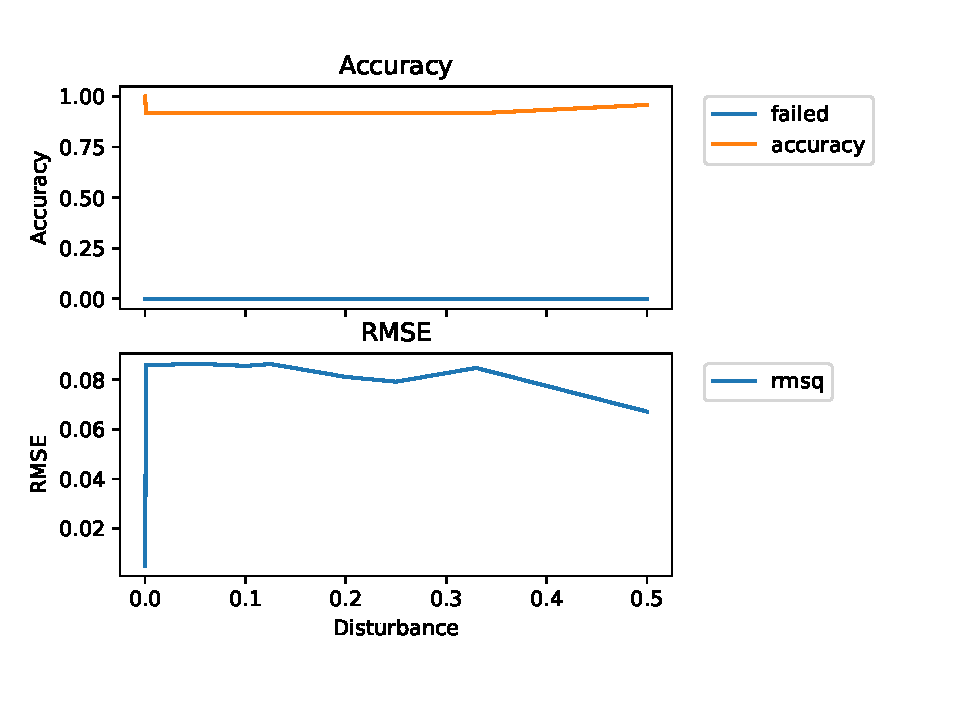
\includegraphics[]{../experiments/GroteMarkt/plots/performance_GroteMarkt.pdf}
\caption{Accuracy (100\% to 0\%) and Root Mean Square error (1 - 0) for rounding to different intervals in GroteMarkt network and simulation}
\label{groteMarkt}
\end{center}
\end{figure}

\subsection{Discussion}

\section{Experiment 2: Swapping out the maps.}
\subsection{Introduction}
What happens if we have the exact same agent logic but we place them in a different spatial configuration? Instead of the Grote Markt, I now put some other part of Groningen in the simulation. We have the same nodes in the network. The only thing that's different is the underlying map.

I selected 5 different parts of Groningen, screenshotted then, converted them to maps like before, and then let the agents loose in them to rob each other.  Then I also made one part just completely empty, and one map random.

\subsection{Methods}

\subsection{Results}

\subsection{Discussion}
Implications of this is that we need to condition explicitly on maps for our networks to work, because it does meaningfully change the probabilities that we find, and there's no way to predict how the map that we're using affects the probabilities. This has implications for the real world, because it means that. ugh. we can't depend on some generic ``probability of getting robbed'', we need to condition on spatial conditions/background world assumptions.

And these are not even very good maps - agents can either go somewhere, or not, and can see through buildings. Affordances in the real world are very different \footnote{parkour!}. So it's likely that the actual probabilities in the real world are even worse...

\section{Experiment 3: Reporters, random variables and the reference class problem}

\subsection{Introduction}
A reporter is a random variable. A random variable maps a sample space to value. Let's make the random variable problematic. What sort of events are we talking about in our sample space? There can be many instantiations of random variables from one natural language string. Here I don't want to talk about the reference class, which is the problem of selecting which sample space we're actually interested in. Instead, it's the awareness that a natural language string (like a node name) by itself does not offer sufficient information to know what events we are actually interested in. We need to select a subset of all the events in the world, that we're actually interested in, and this is underspecified in most bayesian networks.

Some simple \& clear problems

\begin{enumerate}
\item Vlek thesis ``often''. 
\item Fenton simonshaven.
\end{enumerate}

What counts as a relevant event?

For some things its not a problem because in those cases its clear what exactly we're measuring - think DNA evidence, forensic whatever, the node names there are not just natural language strings but they're RVs, a mathematical beast, with an associated method for selecting which events, and the method of knowing whether they're true. We can argue about reference classes and Pardo's barns and Nigerian Smuggler's all day long, but there we have actually established our terms. Here we're talking the step before that. Making the class of interesting events \& the way of knowing that they're true, explicit. They just don't do that in the old research!!! Why not!!!

This has deep implications because if we want BNs to be accepted, everyone relevant in the discussion has to agree exactly on 1) what we're using the nodes `natural language' to mean in RV language, 2) how we're measuring whether an RV is true or not, and then 3) the probability of the RV. I agree with Fenton that subjectivity or slight imprecision in the CPTs in part 3) is ok, fine, as long as everyone knows which parts are subjective. But the greater problems (or at least implicit problems, are 1) and 2), and those need to be made explicit as well.

\subsection{Methods}
I'm going to create many reporters that can all point back to the same natural language meaning. The easiest version is with something inherently subjective like `near', or different definitions of `motive'.

\subsection{Results}

\subsection{Discussion}



\section{Experiment 4: Investigating the island prior - Fenton.}
\subsection{Introduction}

\subsection{Methods}

\subsection{Results}

\subsection{Discussion}

\section{Take aways - Conclusion}


